% !TEX root = sum1.tex
\section{Computational Experiment}\label{sec_result}
We carried out several experiments, including analyzing the performances of different policies, evaluating the impact of implementing social distancing, comparing different layouts, group sizes and social distancing. In the experiment, we set the following parameters. 

% The layout and the values of $M$, $\delta$ will change accordingly as
The default setting in the experiments is as follows, $\delta =1$ and $M =4$. The number of scenarios in SSP is $|\Omega| = 1000$. The default seat layout consists of 10 rows, each with the same size of 21. Different realistic layouts, group sizes and social distances are also explored. We simulate the arrival of exactly one group in each period, i.e., $p_0 = 0$. The average number of individuals per period, denoted as $\gamma$, can be expressed as $\gamma = \sum_{i=1}^{M} i p_i$.

% The occupancy rate at different demands is calculated as the average of these 100 instances. 
% Each entry in the table represents the average performance across 100 instances.

\subsection{Performances of Different Policies}
In this section, we compare the performance of five assignment policies to the optimal one, which can be obtained by solving the deterministic model after observing all arrivals. The policies under examination are DSA, DP-based heuristic, bid-price control, booking limit control and FCFS policy.

\subsection*{Parameters Description}
We consider three sets of probability distributions: D1: [0.18, 0.7, 0.06, 0.06], D2: [0, 0.5, 0, 0.5], D3: [0.2, 0.8, 0, 0], which are experimented in \cite{blom2022filling}. We also consider another probability distribution D4: [0.25, 0.3, 0.25, 0.2] for the extra experiments. To assess the effectiveness of different policies across varying demand levels, we conducted experiments spanning a range of 60 to 100 periods. 

% 我们选择

% [0.12, 0.5, 0.13, 0.25]

% By conducting experiments across this range of periods, we can observe how the different policies perform under both moderate and high-demand situations.

% For the DP Base-heuristic, we consider a simplified dynamic programming by relaxing all rows to a single row with the same total capacity, $\sum_{j=1}^{N} L_j$. With this simplification, we can make decisions for each group arrival based on the relaxed dynamic programming. 

% Bid-price control is a classical approach discussed extensively in the literature on network revenue management. It involves setting bid prices for different group types, which determine the eligibility of groups to take the seats. Specifically, we estimate the bid price of a seat by the shadow price of the capacity constraint in the LP relaxation of problem \eqref{deter_upper}. Then we assign the seats by comparing the revenues of accepting or denying the groups. 

% Booking limit control policy involves setting a maximum number of reservations for each group type. In this policy, we solve problem \eqref{deter_upper} with the expected demand during the time period. Then for every type of requests, we only allocate a fixed amount according to the static solution and reject all other exceeding requests.

The following table presents the performance results of five different policies: DSA, DP, Bid-price, Booking, and FCFS, which stand for dynamic seat assignment, dynamic programming based heuristic, bid-price, booking-limit, and first come first served, respectively. The procedures for the last four policies are detailed in the appendix \ref{policies}. Each entry in the table represents the average performance across 100 instances. Performance is evaluated by comparing the ratio of the number of accepted individuals under each policy to that under the optimal policy, which assumes complete knowledge of all incoming groups before making seat assignments.

\begin{table}[h]
  \centering
  \caption{Performances of Different Policies}
  \begin{tabular}{|c|c|c|c|c|c|c|}
  \hline
  Distribution & T & DSA (\%) & DP (\%) & Bid (\%) & Booking (\%) & FCFS (\%) \\
  \hline
  \multirow{5}{*}{D1} & 60 & 100.00 & 100.00 & 100.00 & 88.56 & 100.00 \\
  & 70    & 99.53 & 99.01 & 98.98 & 92.69 & 98.82 \\
  & 80    & 99.38 & 98.91 & 98.84 & 97.06 & 96.06 \\
  & 90    & 99.52 & 99.23 & 99.10 & 98.24 & 95.37 \\
  & 100   & 99.58 & 99.27 & 98.95 & 98.46 & 94.98 \\
  \hline
  \multirow{5}{*}{D2} & 60  & 99.45 & 97.23 & 96.58 & 99.09 & 96.49 \\
     & 70   & 99.82 & 98.28 & 97.46 & 99.81 & 95.76 \\
     & 80   & 99.92 & 98.60 & 98.86 & 100.00 & 95.66 \\
     & 90   & 99.99 & 99.10 & 99.70 & 100.00 & 95.66 \\
     & 100  & 100.00 & 98.74 & 99.99 & 100.00 & 95.66 \\
  \hline
  \multirow{5}{*}{D3} & 60  & 100.00 & 100.00 & 100.00 & 93.68 & 100.00 \\
     & 70  & 100.00 & 100.00 & 100.00 & 92.88 & 100.00 \\
     & 80  & 99.54 & 97.89 & 97.21 & 98.98 & 96.19 \\
     & 90  & 99.90 & 99.73 & 99.44 & 99.61 & 94.53 \\
     & 100 & 100.00 & 100.00 & 100.00 & 99.89 & 94.32 \\
  \hline
    \multirow{5}{*}{D4} & 60  & 99.61 & 99.68 & 99.63 & 94.01 & 99.61 \\
     & 70  & 99.05 & 98.95 & 98.49 & 97.10 & 96.03 \\
     & 80  & 98.96 & 98.84 & 98.71 & 97.99 & 93.80 \\
     & 90  & 99.38 & 99.17 & 98.70 & 98.36 & 92.87 \\
     & 100 & 99.62 & 99.45 & 99.13 & 98.56 & 92.35 \\
  \hline
  \end{tabular}
\end{table}

We can find that DSA is better than DP-based heuristic, bid-price policy and booking limit policy consistently, and FCFS policy works worst. DP-based heuristic and bid-price policy can only make the decision to accept or deny, cannot decide which row to assign the group to. Booking limit policy does not consider using more seats to meet the demand of one group. FCFS accepts groups in sequential order until the capacity cannot accommodate more.

The performance of DSA, DP-based heuristic, and bid-price policies follows a pattern where it initially decreases and then gradually improves as $T$ increases. When $T$ is small, the demand for capacity is generally low, allowing these policies to achieve relatively optimal performance. However, as $T$ increases, it becomes more challenging for these policies to consistently achieve a perfect allocation plan, resulting in a decrease in performance. Nevertheless, as $T$ continues to grow, these policies tend to accept larger groups, thereby narrowing the gap between their performance and the optimal value. Consequently, their performances improve. In contrast, the booking limit policy shows improved performance as $T$ increases because it reduces the number of unoccupied seats reserved for the largest groups. 

The performance of the policies can vary based on different probabilities. For the different probability distributions listed, DSA performs more stably and consistently for the same demand. In contrast, the performance of DP and bid-price fluctuates more significantly.

% Moreover, according to the results of policies, we can develop an easy-to-implement policy. When $T \leq \frac{\sum_{j}{L_j}}{\gamma + 1}$, we accept the groups based on the first come first served policy. When $T > \frac{\sum_{j}{L_j}}{\gamma + 1}$, we adopt the booking-limit policy, i.e., assign the seats according to the seat planning obtained from problem \eqref{deter_upper}.

% \subsection*{Analysis of DSA}
% We explore the arrival path of one instance under DSA and the optimal solution. The figures show two arrival paths when $T= 55$ and $T= 70$ at the even probability distribution. In the figures, we plot four lines over periods, number of remaining seats, the expected future demand, optimal remaining seats and optimal remaining demand. The horizontal parts of remaining seats represent the rejection at the period. We can observe that when the demand is larger than supply (T =70), even at the beginning we still reject the group. When the demand is lower than supply (T =55), we will accept all groups.

% We also examine the situations where the actual demand is higher or lower than the expected demand.

% Based on the figures provided, we can draw several key conclusions:

% 1. When the demand is larger than supply, even at the very beginning of the time period, both DSA approach and the optimal solution reject some groups, as indicated by the horizontal segments in the lines.

% 2. DSA approach is inclined to accept groups earlier compared to the optimal solution. This is because DSA makes decisions based on the expected future demand, rather than the actual remaining demand.

% 3. When the actual remaining demand is lower than the expected demand, the optimal remaining seats will be lower than that of DSA approach. Conversely, when the actual remaining demand is higher than expected, the optimal remaining seats will be higher than DSA.

% For the DSA, DP Base-heuristic, bid-price policies, their performance tends to initially drop and then increase as the number of periods increases. When the number of periods is small, the demand for capacity is relatively low, and the policies can achieve relatively optimal performance. However, as the number of periods increases, the policies may struggle to always obtain a perfect allocation plan, leading to a decrease in performance. Nevertheless, when the number of periods continue to become larger, these policies tend to accept larger groups, and as a result, narrow the gap with the optimal value, leading to an increase in performance. As the number of periods increases, the performance for the booking limit policy is getting better because the numebr of seats planned for the largest groups that are not occupied will drop.

\subsection{Impact of Social Distancing}
We investigate the impact of social distancing when implementing DSA under varying levels of demand. 
As an illustrative example, we adopt $D4$ as the probability distribution. The demand levels are varied by adjusting the parameter $T$ from 30 to 90 in increments of 1.

% It is evident that as the demand increases, the effect of social distancing becomes more pronounced. We aim to determine the specific time period where the absence of social distancing results in a higher number of accepted individuals compared to when social distancing measures are in place. Additionally, we will calculate the corresponding occupancy rate during this period.

% By analyzing and comparing the data, we can gain insights into the relation between demand, social distancing, the number of accepted individuals, and occupancy rates. This information is valuable for understanding the impact of social distancing policies on overall capacity utilization and making informed decisions regarding resource allocation and operational strategies.

The figure below displays the number of assigned individuals over demand under two different conditions: with social distancing measure and without social distancing measure. For the former case, we employ DSA to obtain the results. In this case, we consider the constraints of social distancing and optimize the seat allocation accordingly. For the latter case, we adopt the optimal solution assuming that all arrivals are known and that there are no social distancing constraints. The figures depicting the results are presented below. The difference between these two figures is the x-axis, the left one is period, while the right one is the percentage of expected demand relative to total seats. 

There are three key points in the figure, the gap point, the target occupancy rate and the maximum achievable occupancy rate.

The gap point $\tilde{T}$ is defined as the largest value of $T$ for which the inequality $E(T; DSA)+1 \geq E(T; OPT)$ holds, where $E(T; DSA)$ denotes the expected number of accepted individuals  across 100 instances by DSA with one seat as social distancing, $E(T; OPT)$ denotes the expected number of accepted individuals across 100 instances by the optimal solution when there is no social distancing. 

The occupancy rate corresponding to the gap point is referred to as the target occupancy rate. This rate represents the maximum demand that can be satisfied under the condition that the difference in the number of accepted individuals remains unaffected by social distancing constraints.

The maximum achievable occupancy rate is defined as $\frac{\sum_{j}\phi(M, L_{j})}{\sum_{j} L_{j}- N \delta}$, where $\phi(M, L)$ indicate the size of any largest pattern under $M$ and $L$. According to the definition of the largest pattern in Proposition \ref{lem_pattern}, $\phi(M, L)$ does not decrease in $M$. Since any largest pattern $\bm{h}$ under $M$ is a feasible pattern under $(M+1)$, then, $\phi(M, L) \leq \phi(M+1, L)$. Therefore, when $M$ increases and $L$ is unchanged, the maximum achievable occupancy rate increases.

Sometimes, the policy also requires a maximum allowable occupancy rate to tighten the social distancing requirement. The maximum allowable rate will be redundant if it is higher than the maximum achievable rate for all events. Only the requirement on occupancy rate is effective and the requirement on social distancing is not effective for an event if it is lower than the target occupancy rate of the event. Furthermore, when the maximum allowable rate is between the target occupancy rate and the maximum achievable rate, the requirements on seat occupancy and social distancing interact to determine the seat assignment.


% Similarly, $\phi(M, L)$ does not decrease in $L$. Since any largest pattern $\bm{h}$ under $L$ is a feasible pattern under $L+1$, thus, $\phi(M, L) \leq \phi(M, L+1)$.

\begin{figure}[h]
  \centering
  \subfigure[]{
    \label{x_period}
    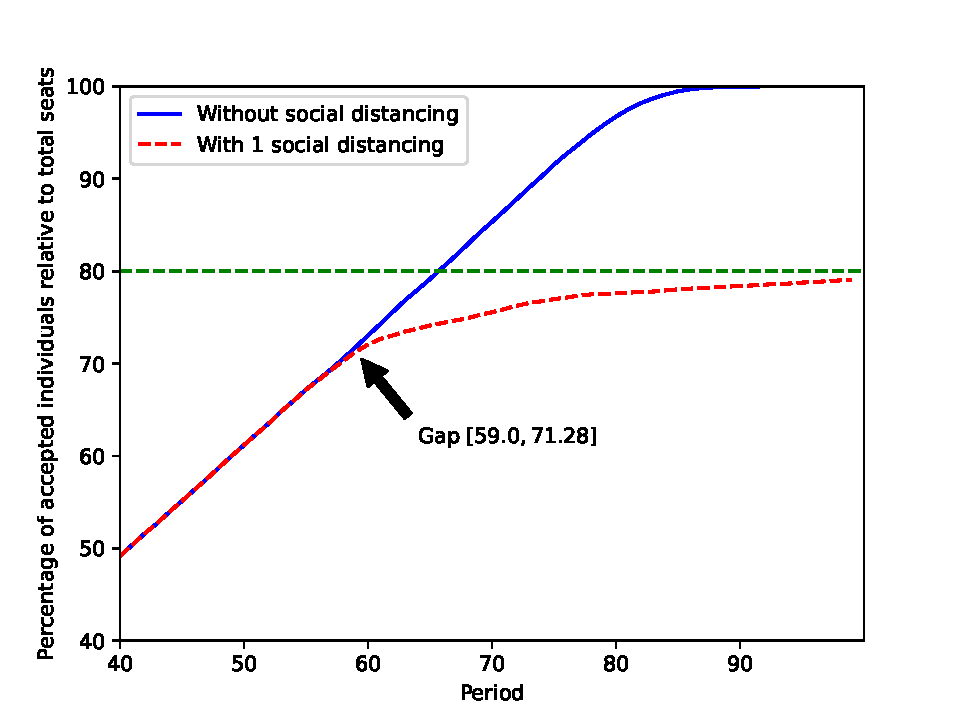
\includegraphics[width=0.48\textwidth]{./Figures/occu_demand_group4.pdf}}
  \subfigure[]{
    \label{x_demand}
    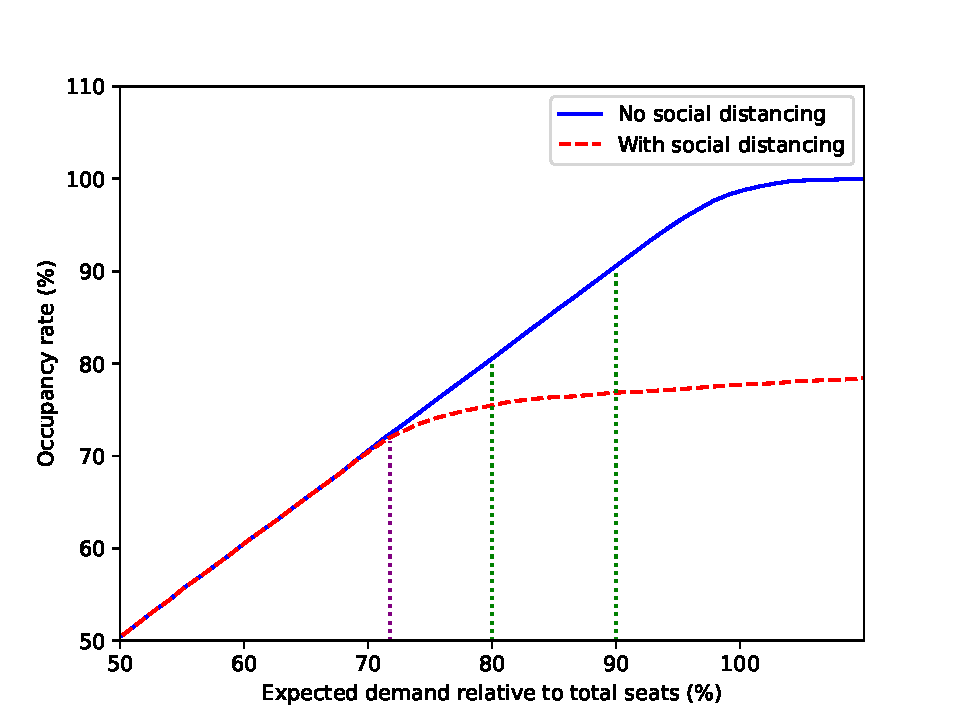
\includegraphics[width=0.48\textwidth]{./Figures/occu_gamma_group4.pdf}}
  \caption{The occupancy rate over demand}
  \label{occupancy_rate_demand}
\end{figure}

% Intuitively, when demand is low, we will accept all arrivals, and there will be no difference in the number of accepted individuals whether we implement social distancing or not. The interesting case is when the difference in the number of accepted individuals due to social distancing starts to occur.

In the first figure, the gap point is 60, the target occupancy rate is 71.8\%. As the expected demand continues to increase, both situations reach their maximum capacity acceptance. For the social distancing situation, when the largest pattern is realized in each row, the maximum achievable occupancy rate is given by $\frac{16}{20} = 80\%$. The second figure is plotted to show that when the expected demand is less than 71.8\%, the social distancing measures will not have an impact; when the expected demand is larger than 71.8\%, the difference between the number of accepted individuals with and without social distancing measures becomes more pronounced. 

% The policy requires a maximum allowable occupancy rate larger than 80\% will be redundant.

\subsection{Estimation of Gap Points}
To estimate the gap point, we aim to find the maximal period such that all requests can be assigned into the seats during these periods, i.e., for each group type $i$, we have $\bm{X}_{i} = \sum_{j} x_{ij} \geq d_i$. Meanwhile, we have the capacity constraint $\sum_{i} n_{i} x_{ij} \leq L_j$, thus, $\sum_{i} n_i d_i \leq \sum_{i} n_i \sum_{j} x_{ij} \leq \sum_{j} L_{j}$. Notice that $E(d_i) = p_i T$, we have $\sum_{i} n_i p_i T \leq \sum_{j} L_{j}$ by taking the expectation. Recall that $\tilde{L} = \sum_{j} L_{j}$ denotes the total number of seats, and $\gamma$ represents the average number of individuals in each period. Then, we can derive the inequality $T \leq \frac{\tilde{L}}{\gamma + \delta}$. Therefore, the upper bound for the expected maximal period is given by $T' = \frac{\tilde{L}}{\gamma + \delta}$.


Assuming that all arrivals within $T'$ periods are accepted and fill all the available seats, the target occupancy rate can be calculated as $\frac{\gamma T'}{(\gamma+ \delta)T' - N \delta} = \frac{\gamma}{\gamma +\delta} \frac{\tilde{L}}{\tilde{L}-N \delta}$. However, it is important to note that the actual maximal period will be smaller than $T{'}$ because it is nearly impossible to accept groups to fill all seats exactly. To estimate the gap point when applying DSA, we can use $y_1 = c_1 \frac{\tilde{L}}{\gamma + \delta}$, where $c_1$ is a discount factor compared to the ideal assumption. Similarly, we can estimate the target occupancy rate as $y_2 = c_2 \frac{\gamma}{\gamma +\delta} \frac{\tilde{L}}{\tilde{L}-N \delta}$, where $c_2$ is a discount factor for the occupancy rate compared to the ideal scenario.

To analyze the relation between $\gamma$ and the gap point, we conducted an analysis using a sample of 200 probability distributions. The figure below illustrates the gap point as a function of $\gamma$, along with the corresponding estimations.  Additionally, the target occupancy rate is represented by red points. 
% For each probability distribution, we considered 100 instances and plotted the gap point as blue points.
We applied an Ordinary Least Squares (OLS) model to fit the data and estimate the parameter values. The resulting fitted equations, $y_1 = \frac{c_1 \tilde{L}}{\gamma + \delta}$ (represented by the blue line in the figure) and $y_2 = c_2 \frac{\gamma}{\gamma + \delta} \frac{\tilde{L}}{\tilde{L}-N \delta}$ (represented by the orange line in the figure), are displayed in the figure. The goodness of fit is evaluated using R-squared values, which are 1.000 for both models, indicating a perfect fit between the data and the fitted equations. The estimated discount factor values are $c_1 = 0.9578$ and $c_2 = 0.9576$.

\begin{figure}[ht]
  \centering
    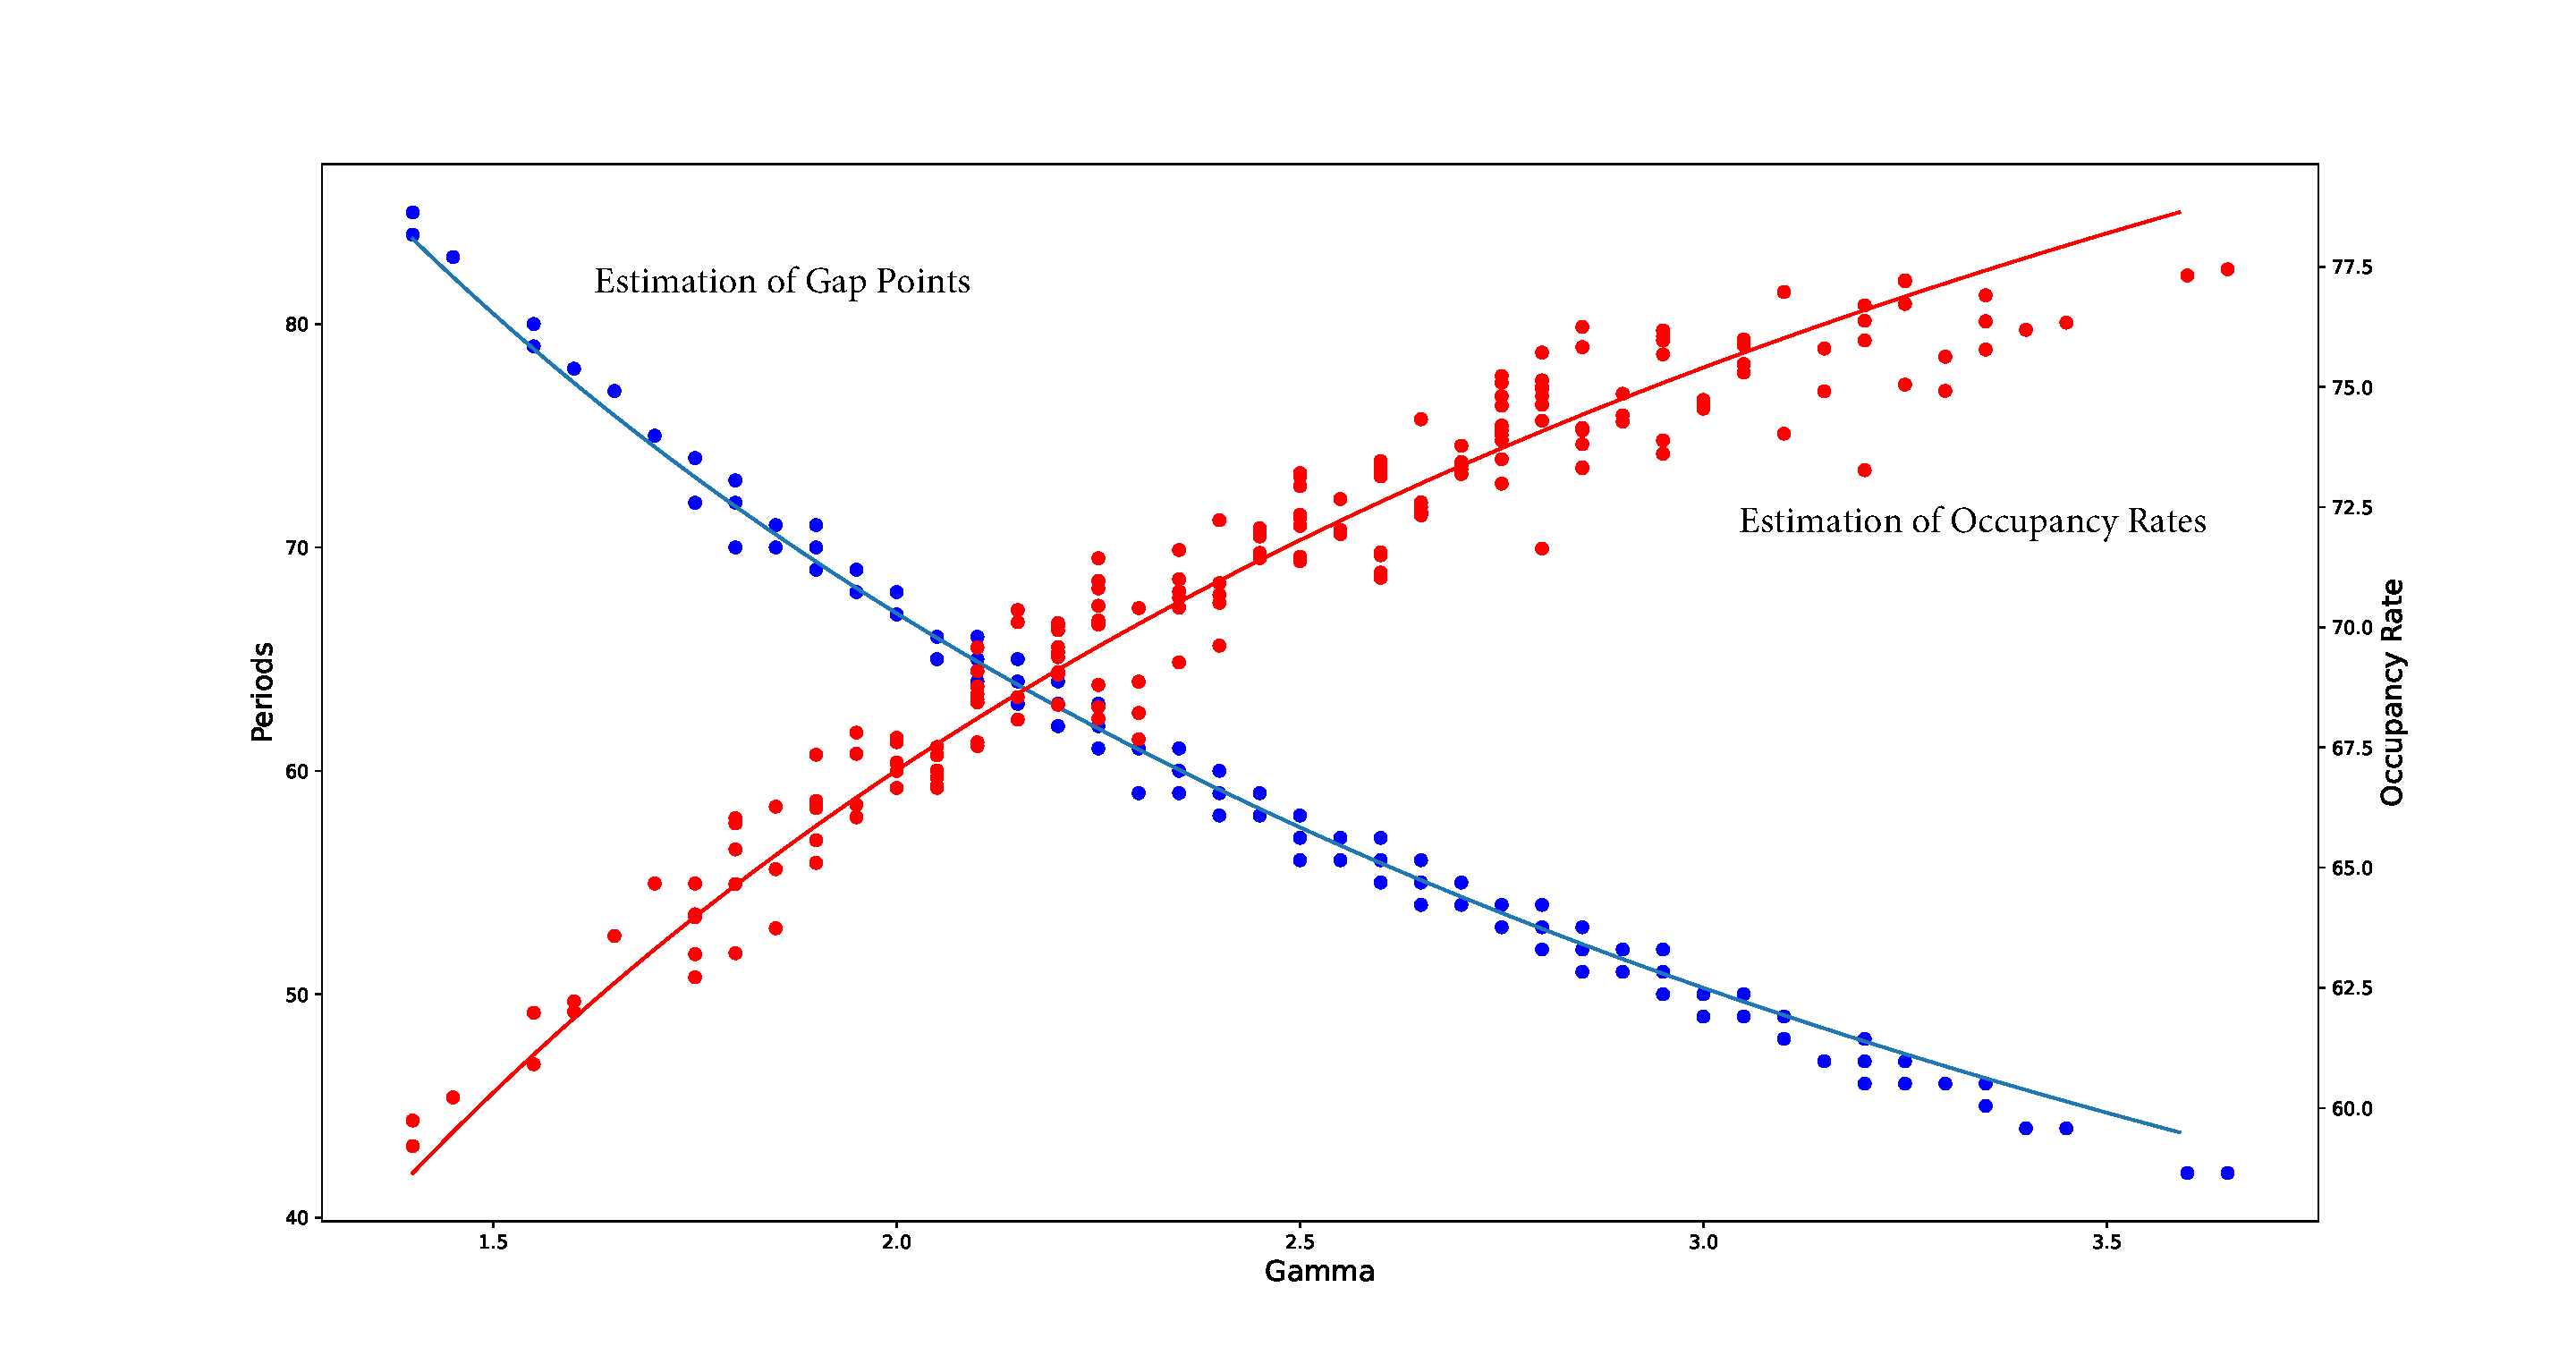
\includegraphics[width=0.95\textwidth]{./Figures/gamma_estimation.pdf}
  \caption{Gap points and their estimation under 200 probabilities}
\end{figure}

% As the value of $\gamma$ increases, the gap point will decrease and the corresponding occupancy rate will increase. Consequently, the occupancy rate increases due to the allocation of seats to larger groups. The percentage difference is negligible when the demand is small, but it becomes more significant as the demand increases.

Based on the above analysis, we also explore the results of different layouts, different group sizes and different social distances. Since the figure about the occupancy rate over demand is similar to Figure \ref{occupancy_rate_demand}, we only use three metrics to show the results: the gap point and the target occupancy rate, maximal achievable occupancy rate.

\subsection*{Different Layouts}
We experiment with several realistic seat layouts selected from the theater seat plan website, https://www.lcsd.gov.hk/en/ticket/seat.html. We select five places, Hong Kong Film Archive Cinema, Kwai Tsing Theatre Transverse Stage, Sai Wan Ho Civic Centre, Sheung Wan Civic Centre, Ngau Chi Wan Civic Centre, represented as HKFAC, KTTTS, SWHCC, SWCC, NCWCC respectively. HKFAC, SWCC, NCWCC, are approximately rectangular layouts, SWHCC is a standard rectangular layout. While KTTTS is an irregular layout.


In these layouts, wheelchair seats and management seats are excluded, while seats with sufficient space for an aisle are treated as new rows. 

% The same 100 instances with the probability of $D4$ are experimented for each layout.

The occupancy rate over demand follows the typical pattern of Figure \ref{occupancy_rate_demand}. The gap point, the target occupancy rate and the maximum achievable occupancy rate are also given in the following table. The maximum achievable occupancy rate can be calculated from Proposition \ref{lem_pattern}.

\begin{table}[ht]
  \centering
  \caption{Gap points and target occupancy rates of the layouts}
  \begin{tabular}{|c|c|c|}
  \hline
   Seat Layout & Gap point & Target occupancy rate  \\
   \hline
   HKFAC & 37 & 70.63 \%  \\
   KTTTS & 40 & 75.64 \%   \\
   SWHCC & 33 & 71.31 \%  \\
   SWCC & 45 & 73.57 \%   \\
   NCWCC & 105 & 72.05 \%  \\
   \hline
  \end{tabular}
\end{table}


Generally speaking, the length of each row impacts the occupancy rate, as a full pattern can maximize seat utilization, leading to a higher occupancy rate. However, in rectangular layouts, achieving a full pattern in each row can be challenging, resulting in a relatively low occupancy rate, as seen in SWHCC. Although these layouts are all approximately rectangular, the varying lengths of each row lead to different occupancy rates, as demonstrated by HKFAC, SWCC, and NCWCC.

% This suggests that, when the total number of seats is the same, the layout with more rows yields a larger gap point and occupancy rate compared to the layout with fewer rows.

% For each row, a seat is designated for social distancing with every group accepted. Consequently, when each row follows a full pattern and the total number of seats remains constant, having more rows results in a higher gap point and occupancy rate. Similarly, in a small room with fewer seats per row, the occupancy rate at the gap point will correspondingly be higher.

\subsection*{Different Group Sizes}
For group sizes of 3, 4 and 5, we present the gap point, the target occupancy rate and the maximum achievable occupancy rate in the table below. The probability distributions for these group sizes all share the same value of $\gamma = 2.4$.

\begin{table}[ht]
  \centering
  \caption{Gap points and target occupancy rates of the group sizes}
  \begin{tabular}{|c|c|c|c|}
  \hline
   Group Size & Probability distribution & Gap point & Target occupancy rate \\
  \hline
   3 & [0.2, 0.2, 0.6] & 60.0  & 71.83 \%  \\
   4 & [0.25, 0.3, 0.25, 0.2] & 60.0 & 71.79 \%   \\ 
   5 & [0.3, 0.3, 0.2, 0.1, 0.1] & 58.0 & 70.00 \% \\
   \hline
  \end{tabular}
\end{table}

% We observe that larger group sizes correspond to higher largest occupancy rates under the same seat layout. However, the gap point and occupancy rate for larger group sizes do not necessarily increase correspondingly. The explanation for this is that as larger groups are allowed to be accepted, seat allocation makes it difficult to achieve a full pattern for each row. Thus, there will be a decrease in both gap points and occupancy rates, i.e., the impact of social distancing will manifest at an earlier period.

% The insight is although allowing larger groups will increase the largest occupancy rate, the impact of social distancing will become evident at an earlier period. Specifically, if demand is low or if the managers wish to avoid rejecting a significant number of customers, they can set a smaller group size limit. Conversely, when demand is high, a larger group size limit can be set to accommodate more customers.

\subsection*{Different Social Distances}
The following figure illustrates the number of accepted individuals over time with social distancing set at 0, 1, and 2 seats, respectively.

\begin{figure}[h]
  \centering
    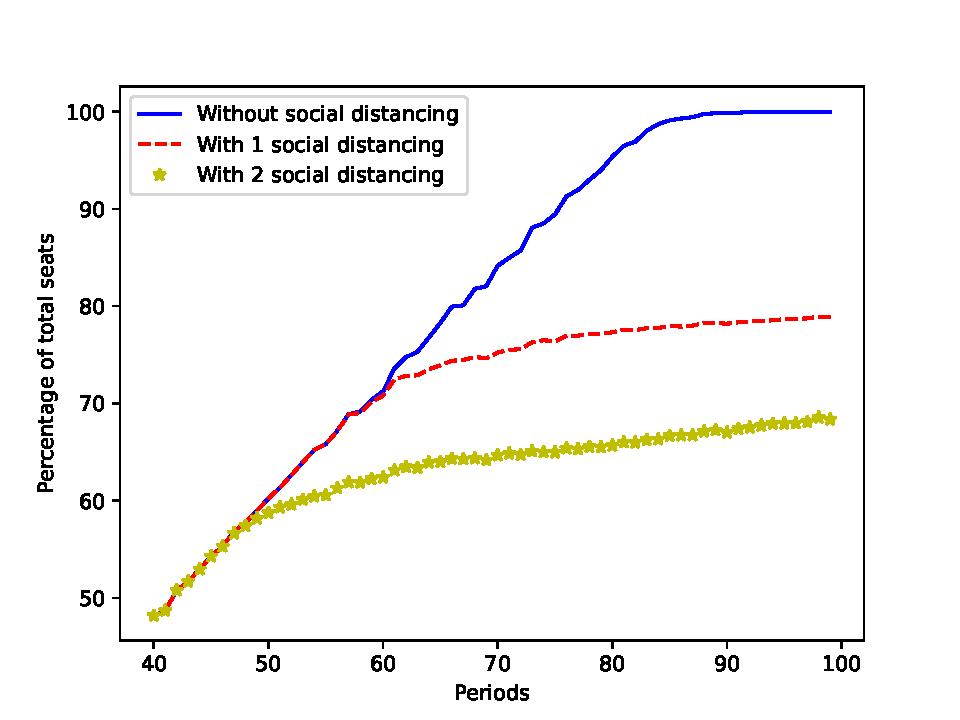
\includegraphics[width=0.8\textwidth]{./Figures/distance.pdf}
  \caption{The occupancy rate over demand for different social distancings}
\end{figure}


% We examine the impact of implementing social distancing on the occupancy rate and explore strategies to minimize revenue loss. Consider the situation where the gap point is $\tilde{T}$ and is determined by the parameters $\delta$, $\gamma$, $M$, and $\tilde{L}$. The corresponding occupancy rate is $\Gamma(\tilde{T})$. When the actual number of people (demand) is less than $\tilde{L} \cdot \Gamma(\tilde{T})$, implementing social distancing does not affect the revenue. However, if the actual number of people exceeds $\tilde{L} \cdot \Gamma(\tilde{T})$, enforcing social distancing measures will lead to a reduction in revenue. The extent of this loss can be assessed through simulations by using the specified parameters. To mitigate the potential loss, the seller can increase the value of $\gamma$. This can be achieved by implementing certain measures, such as setting a limit on the number of single-person groups or allowing for larger group sizes. 


At times, the government may establish a maximum allowable occupancy rate. This rate is effective for an event only if it is lower than the expected occupancy rate. Additionally, the maximum allowed rate becomes redundant if it exceeds the maximum achievable rate for all events.


% for example, for family movies in cinemas, $\gamma$ will be relatively large, so a higher occupancy rate limit can be set.




% HONG KONG FILM ARCHIVE CINEMA [17, 18, 18, 18, 18, 18, 18, 8]

% Kwai Tsing Theatre Transverse Stage [7, 9, 7, 10, 7, 11, 8, 11, 9, 7, 10, 7, 11, 7, 13, 8]

%%  Kwai Tsing Theatre Arena Stage  [6, 6, 5, 7, 7, 7, 8, 8, 7, 7, 7, 7, 8, 8, 6, 4, 5, 5, 6, 6, 6, 6, 4, 6, 5, 5, 6, 6, 6, 6]

% Sai Wan Ho Civic Centre [6, 6, 6, 6, 6, 6, 6, 6, 6, 6, 6] 6* 22

% Sheung Wan Civic Centre [3, 13, 13, 13, 13, 13, 13, 13, 13, 13, 13, 13, 13]

% Ngau Chi Wan Civic Centre Theatre  [13, 21, 23, 23, 23, 23, 23, 23, 23, 23, 23, 23, 23, 23, 23, 21, 13]